To address the gap in table-to-text generation for user-specific aspects or queries, such as ``Camera'' and ``Design \& Display'' (as illustrated in Figure \ref{fig:task-def}), we developed the \textbf{eC-Tab2Text} dataset. This dataset comprises e-commerce product tables and is designed to facilitate aspect-based text generation by fine-tuning LLMs on our dataset. The pipeline for creating \textbf{eC-Tab2Text} is outlined in Figure \ref{fig:data-pipeline} and described in detail below.

\begin{figure}[H]
    \centering
    \includegraphics[width=10cm]{images/eC-Tab2Text.pdf}
    \caption{eC-Tab2Text Dataset Pipeline}
    \label{fig:data-pipeline}
\end{figure}

The methodology is summarized in a flowchart (Figure \ref{fig:MethodologyFlowchart}). This structured approach guarantees a comprehensive and reproducible pathway for leveraging LLMs to transform structured product data into human-readable reviews while addressing challenges such as data sparsity and domain-specific needs.
\begin{figure}[H]
    \centering
    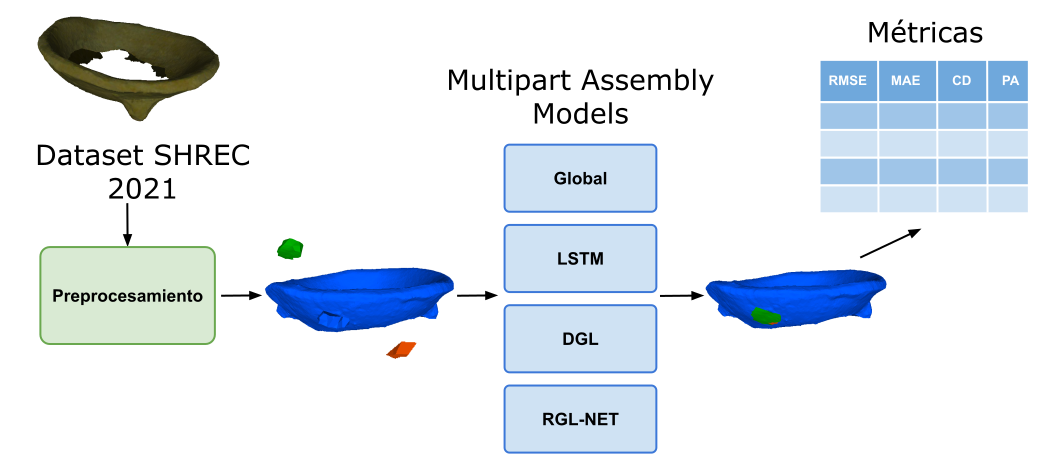
\includegraphics[width=10cm]{images/Methodology.jpg}
    \caption{Methodology Flowchart}
    \label{fig:MethodologyFlowchart}
\end{figure}
